\documentclass[12pt]{article}

%% preamble: Keep it clean; only include those you need
\usepackage{amsmath}
\usepackage[margin = 1in]{geometry}
\usepackage{graphicx}
\usepackage{booktabs}
\usepackage{natbib}
% for space filling
\usepackage{lipsum}
% highlighting hyper links
\usepackage[colorlinks=true, citecolor=blue]{hyperref}
\usepackage{tabularx}
\usepackage{adjustbox}

%% meta data

\title{Bridging Gaps: Investigating COVID-19's Influence on Health Disparities in Connecticut}
\author{Delia Lin\\
  Department of Statistics\\
  University of Connecticut
}

\begin{document}
\maketitle

\begin{abstract}
    Social determinants of health (SDOH) are the conditions in which people are born, 
    grow, live, work, and age, which significantly influence their overall health and 
    well-being. These determinants include factors such as socioeconomic status, education, 
    access to healthcare, and the physical environment. Understanding the interactions of 
    these elements will be essential for addressing health disparities and developing more 
    effective public health policies and interventions.  
\end{abstract}

\section{Introduction}\label{sec:intro}


Current research focuses on how social determinants of health (SDoH) plays a  massive
impact on one's health; it is estimated that 80 percent of a population's health outcomes are 
dictated by SDoH \citep{HOOD2016129}. Often, SDoH, when referring to an individual, can result in racial 
disparities in care when looking at a population\citep{Monroe2023-uq}. It has been shown that major inefficiencies
in the health system are attributed to overlooked prevention opportunities and unequal access
to care.\citep{Allin2014-xn}

Understanding the intricate interplay of these social determinants is crucial in addressing health disparities 
and developing effective public health policies and interventions. The COVID-19 pandemic has shed new light on 
these disparities, amplifying existing inequalities within various communities. This research topic gains paramount 
importance in the current context as it seeks to delve into the specific impact of COVID-19 on key social determinants 
of health in different counties and racial groups in Connecticut.

The existing literature underscores the pressing need for research in this area. Studies have shown that predominantly 
black counties in the United States experience significantly higher COVID-19 infection and mortality rates, emphasizing 
the racial disparities prevalent in healthcare outcomes. The pandemic has magnified these discrepancies, leading to 
mortality rates among historically marginalized minority communities that are 1.9 to 2.4 times higher compared to the 
general population \citep{Badalov2022-wt}. Additionally, inefficiencies in the healthcare system have been attributed 
to overlooked prevention opportunities and unequal access to care, necessitating a comprehensive examination 
of these social determinants in the context of the pandemic.

Despite the growing body of research on SDOH, there is a notable gap concerning the specific impact of COVID-19 on 
these determinants within diverse communities. This research aims to bridge this gap by comprehensively assessing how 
the pandemic has influenced key social determinants of health across various counties and racial groups in Connecticut. 
By identifying the specific ways in which different communities were affected, this study contributes valuable insights 
for targeted interventions, policy-making, and the development of equitable healthcare strategies.


% roadmap
The rest of the paper is organized as follows.

The data will be presented in Section\ref{sec:data}

The methods are described in Section\ref{sec:meth}

The results are reported in Section\ref{sec:resu}

A discussion concludes in Section\ref{sec:disc}

\section{Methods}\label{sec:meth}

In this study, descriptive statistics is utilized to outline the total population, racial composition, 
education levels, and average rehospitalization rate across the 8 counties in Connecticut. ANOVA tests were 
conducted to assess the significance of the difference of the variables of median income, poverty level, health insurance, 
utilities access, and electronics access between counties and across the four years (2017, 2018, 2019, 2020). Additional 
Tukey's HSD tests were conducted to determine the specific counties and years that have had significant differences within 
each of the variables for each county.

\section{Data}\label{sec:data}

Data was collected from The Agency for Healthcare Research and Quality (AHRQ).The dataset comprises 7 variables 
spanning a period of 4 years (2017, 2018, 2019, 2020) with observations across the 8 counties in Connecticut. These variables 
encompass a total of 56 observations. The variables questions include housing, education level, income, insurance,
rehospitalization rates, food stamps usage, and population racial characteristics. The dataset includes a range of 
calculated percentages, median values, and raw observations, providing a holistic view of various factors affecting 
the communities in these counties. 


\section{Results}\label{sec:resu}


\begin{table}[]
  \resizebox{\columnwidth}{!}{%
  \begin{tabular}{lllllllllllllll}
                            &                                              &                  &                 &                   &                  &                  &                   &                &                &  &  &  &  &  \\
  \textbf{County}           &                                              & Fairfield County & Hartford County & Litchfield County & Middlesex County & New Haven County & New London County & Tolland County & Windham County &  &  &  &  &  \\
  \textbf{Total Population} &                                              & 944977           & 894465.25       & 182657.5          & 163318.25        & 858678           & 268477.75         & 151218.75      & 116608.75      &  &  &  &  &  \\
  \textbf{Race}             & American Indian and Alaska Native race alone & 0.24             & 0.3075          & 0.2025            & 0.195            & 0.1725           & 0.605             & 0.05           & 0.565          &  &  &  &  &  \\
                            & Asian                                        & 5.2925           & 5.2925          & 1.9               & 3.0625           & 4.005            & 4.12              & 4.675          & 1.3675         &  &  &  &  &  \\
                            & Black or African American                    & 11.405           & 13.7025         & 1.83              & 5.385            & 13.34            & 5.8175            & 3.1075         & 2.33           &  &  &  &  &  \\
                            & Native Hawaiian and Pacific Islander         & 0.055            & 0.035           & 0                 & 0.005            & 0.0225           & 0.025             & 0              & 0.015          &  &  &  &  &  \\
                            & White                                        & 72.6325          & 70.67           & 92.6025           & 88.0875          & 73.2875          & 80.6175           & 88.025         & 88.8725        &  &  &  &  &  \\
  \textbf{Ethnicity}        & Hispanic                                     & 19.53            & 17.8275         & 6.15              & 6.12             & 17.885           & 10.5              & 5.4475         & 11.6375        &  &  &  &  &  \\
  \textbf{Education}        & Associates                                   & 20.74            & 25              & 27.9225           & 26.46            & 24.4175          & 29.2675           & 26.315         & 30.9775        &  &  &  &  &  \\
                            & Bachelor                                     & 26.53            & 21.4575         & 20.635            & 23.3325          & 18.785           & 18.3175           & 23.4075        & 14.595         &  &  &  &  &  \\
                            & Graduate Degree                              & 21.14            & 16.475          & 14.6975           & 18.4525          & 16.3425          & 15.18             & 17.865         & 9.55           &  &  &  &  &  \\
                            & HS Graduate                                  & 21.4725          & 26.7175         & 29.5875           & 26.0275          & 30.565           & 29.46             & 27.03          & 33.5125        &  &  &  &  &  \\
                            & Less the High School                         & 10.12            & 10.3525         & 7.1575            & 5.7275           & 9.8875           & 7.7725            & 5.385          & 11.365         &  &  &  &  &  \\
                            &                                              &                  &                 &                   &                  &                  &                   &                &                &  &  &  &  & 
  \end{tabular}%
  }
  \end{table}
    




\begin{figure}[tbp]
  \centering
  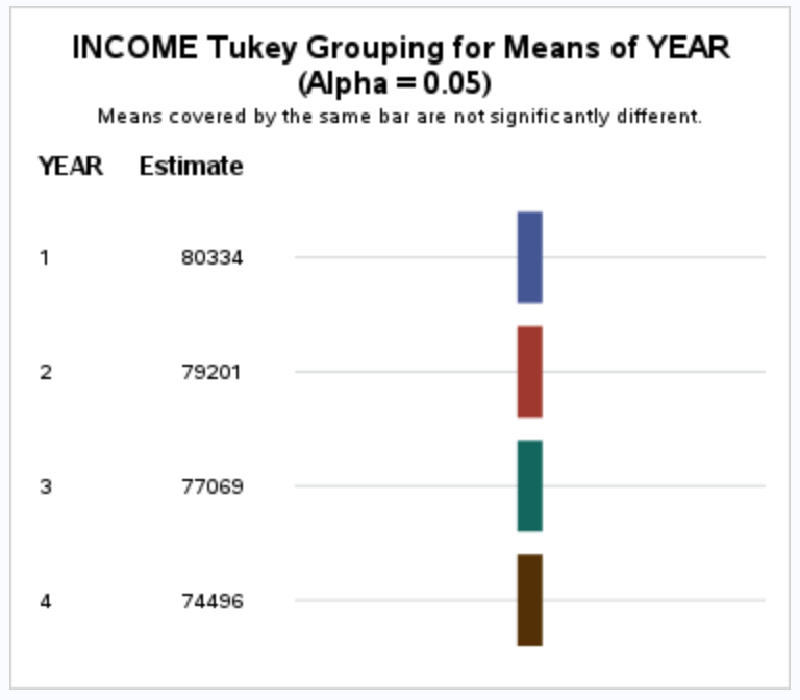
\includegraphics[width=\textwidth]{Income by year.pdf}
  \caption{Median Income by Year.}\label{fig:cars}
\end{figure}

\begin{figure}[tbp]
    \centering
    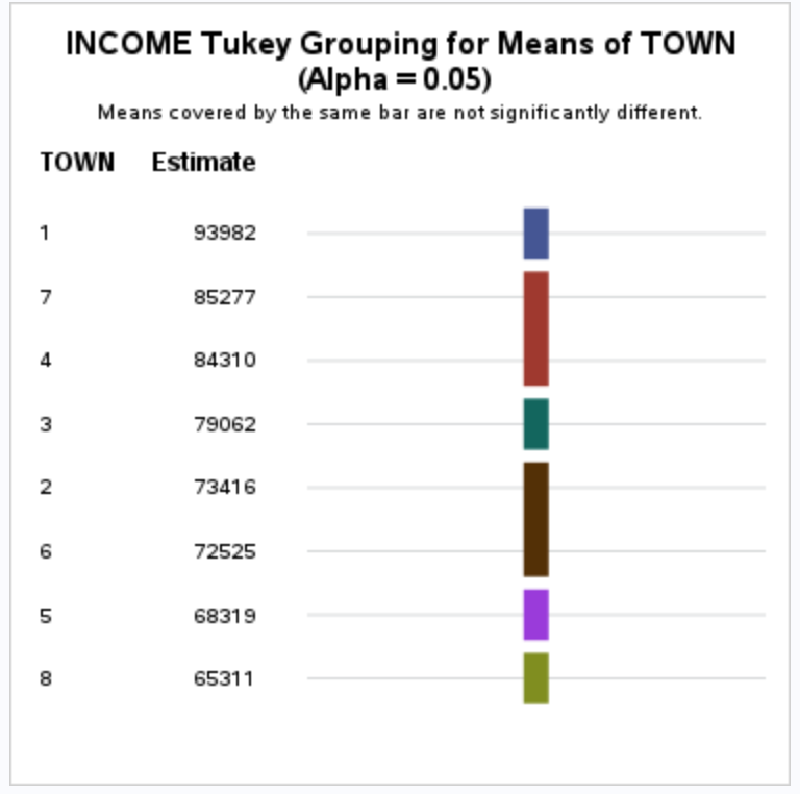
\includegraphics[width=\textwidth]{Income by town.pdf}
    \caption{Median Income by County.}\label{fig:cars}
  \end{figure}

\section{Discussion}\label{sec:disc}

The results of the analysis shed light on the intricate relationships between county, race, and key 
variables such as median income, housing affordability, rehospitalization rates, food stamps usage, 
uninsured rates, and racial demographics. Understanding these correlations is vital in comprehending 
the socio-economic and racial disparities prevalent in the studied region.

The disparity in median income over the studied years, particularly the peak observed in 2020, 
signifies economic fluctuations. Notably, county 1 stands out with significantly higher income 
compared to other counties, indicating potential disparities in resource access and opportunities. 
This wealth gap implies potential repercussions on community health outcomes. The consistent trend in 
the percentage of income spent on rent underscores a persistent challenge for residents, especially 
noticeable in counties 1 and 5, indicating enduring economic pressure.

Rehospitalization rates demonstrate stability across counties and years leading up to 2020, suggesting 
a consistent healthcare landscape. Counties 8, 2, and 5 exhibiting higher food stamp usage point to economic 
challenges faced by residents in these regions. This trend aligns with housing affordability issues, 
indicating a correlation between financial stress and reliance on government assistance programs.

The notably high uninsured rate in county 1 raises concerns about healthcare accessibility, likely 
linked to economic factors impacting insurance affordability. Conversely, the lower uninsured rate in 
Year 3 (2019) signifies positive progress. Analyzing the policies or interventions implemented during 
this period could provide valuable insights for effective healthcare reforms, offering potential guidance 
for future initiatives.

\subsubsection{Racial Disparities}
The racial demographics highlight disparities in various counties. County 3's higher percentage of white 
individuals, coupled with County 2, 5, and 1 having the highest black population, points to the need for
targeted interventions addressing racial health inequalities. These disparities might be indicative of 
historical, social, and economic factors influencing the healthcare experiences of different racial groups.

\subsection{Limitations}
One limitation lies in the availability and quality of data. This dataset does not have any 
data from years after 2020 which may serve to limit potential external validity considerations. 
There may also be variability in data collection methods and discrepancies in reporting standards 
leading to missing or incomplete data over the course of 4 years. Another limitation involves the scope 
of the study, focusing on specific counties in Connecticut may not fully capture nationwide disparities. 
Additionally, the research is limited to the factor parameters selected to investigate which  might not 
encompass all relevant social determinants affecting health outcomes.

\subsection{Future Directions}
These findings underscore the complex interplay between socio-economic status, race, and health outcomes. 
Addressing these disparities requires multifaceted interventions, including economic support, affordable 
housing initiatives, and targeted healthcare access programs. Future research should delve deeper into the 
root causes of these disparities, considering historical and systemic factors. Additionally, policy interventions 
and community-based programs should be designed to specifically target areas and populations facing the most 
significant challenges, aiming for a more equitable healthcare landscape for all residents.


\appendix

\bibliography{../manuscript/ref}
\bibliographystyle{chicago}

\end{document}

{housing by income.pdf}
{housing by year.pdf}
{Income by town.pdf}
{Inome by year.pdf}
{Rehosp by income/year.pdf}
{Stamps by income/year.pdf}